
\subsection*{Đề thi thử THPTQG 2026 - Lần 1 - Trường THPT chuyên Lê Thánh Tông - Đà Nẵng }%% Sở GDDT Đà Nẵng - THPT chuyên Lê Thánh Tông 2026
\Opensolutionfile{ans}[ans/ans-OTTNTHPT-DE27-LC]
\caulc
\begin{ex}%[2H2N2-2]
	Trong không gian $Oxyz$, cho điểm $M(1;2;3)$. Tìm tọa độ hình chiếu của $M$ lên trục $Ox$.
	\choice
	{$(2;0;0)$}
	{$(0;2;3)$}
	{$(3;0;0)$}
	{\True $(1;0;0)$}
	\loigiai{
		Hình chiếu của điểm $M(1;2;3)$ lên trục $Ox$ có tung độ và cao độ bằng $0$, giữ nguyên hoành độ.		
		Vậy hình chiếu là $(1;0;0)$.
	}
\end{ex}

\begin{ex}%[1D2N3-4]
	Cấp số nhân $(u_n)$ có $u_1=9,\ u_2=3$. Số hạng $u_5$ của cấp số nhân là
	\choice
	{$u_5=243$}
	{$u_5=81$}
	{\True $u_5=\dfrac{1}{9}$}
	{$u_5=\dfrac{1}{81}$}
	\loigiai{
		Ta có
		$
		q=\dfrac{u_2}{u_1}=\dfrac{3}{9}=\dfrac{1}{3}
		$		
		suy ra
		$
		u_5=u_1q^4
		=9\cdot\left(\dfrac{1}{3}\right)^4
		=\dfrac{1}{9}.
		$
	}
\end{ex}

\begin{ex}%[2H2N2-4]
	Trong không gian với hệ trục tọa độ $Oxyz$, cho các điểm	
	$A(1;3;2)$, $B(1;0;1)$, $C(5;-3;2)$.	
	Biết rằng $\vec{AB}\cdot\vec{AC}=2m$. Giá trị của $m$ là
	\choice
	{$m=-9$}
	{$m=-18$}
	{\True $m=9$}
	{$m=18$}
	\loigiai{
		Ta có
		$\vec{AB}=(0;-3;-1)$,
		$\vec{AC}=(4;-6;0)$
		suy ra
		$\vec{AB}\cdot\vec{AC}
		=0\cdot4+(-3)(-6)+(-1)\cdot0
		=18$.\\		
		Do $\vec{AB}\cdot\vec{AC}=2m$ nên
		$
		2m=18\Rightarrow m=9.
		$
	}
\end{ex}

\begin{ex}%[1D6H2-1]
	Cho $0<a\ne1$. Giá trị của biểu thức
	$
	P=\log_{a}\left(a\cdot\sqrt[3]{a^2}\right)
	$
	là
	\choice
	{ $a^{\tfrac{5}{3}}$}
	{\True $\dfrac{5}{3}$}
	{$\dfrac{4}{3}$}
	{$\dfrac{5}{2}$}
	\loigiai{
		Ta có
		$a\cdot\sqrt[3]{a^2}=a^{\tfrac{5}{3}}$	
		suy ra
		$P=\log_{a}\left(a\cdot\sqrt[3]{a^2}\right)=\dfrac{5}{3}$.
		}
\end{ex}

\begin{ex}%[2D1H4-1]
	Đường cong trong hình vẽ bên là đồ thị của hàm số nào?
	\immini{\choice
		{$y=\dfrac{2x-1}{x-1}$}
		{\True$y=\dfrac{x+1}{x-1}$}
		{$y=\dfrac{2x-2}{2x+1}$}
		{$y=\dfrac{-x+1}{x+1}$} }
	{
	\begin{tikzpicture}[>=stealth,scale=0.5]
		
		\draw[->] (-4,0)--(5,0) node[right]{$x$};
		\draw[->] (0,-4)--(0,5) node[above]{$y$};
		
		\draw[dashed] (1,-4)--(1,5);
		\draw[dashed] (-4,1)--(5,1);
		
		\node[below right] at (1,0) {$1$};
		\node[above left] at (0,1) {$1$};
		\node[below right] at (0,0) {$O$};
		
		\draw[smooth,domain=-4:0.6,samples=200]
		plot(\x,{(\x+1)/(\x-1)});
		
		\draw[smooth,domain=1.5:5,samples=200]
		plot(\x,{(\x+1)/(\x-1)});		
	\end{tikzpicture}}
	\loigiai{
		Quan sát đồ thị thấy có tiệm cận đứng $x=1$ và tiệm cận ngang $y=1$.
		Trong các đáp án chỉ có hàm số
		\[
		y=\dfrac{x+1}{x-1}
		\]
		thỏa mãn.
	}
\end{ex}

\begin{ex}%[2D3H1-3]
	Thời gian truy cập Internet mỗi buổi tối của một số học sinh được cho trong bảng
	\begin{center}
		\begin{tabular}{|c|c|c|c|c|c|}
			\hline
			Thời gian (phút) & $[9{,}5;12{,}5)$ & $[12{,}5;15{,}5)$ & $[15{,}5;18{,}5)$ & $[18{,}5;21{,}5)$& $[21{,}5;24{,}5]$\\
			\hline
			Số học sinh & $3$ & $12$ & $15$ & $24$&$2$\\
			\hline
		\end{tabular}
	\end{center}
	Tứ phân vị thứ ba $Q_3$ của mẫu số liệu ghép nhóm bằng
	\choice
	{\True $20$}
	{$21$}
	{$18{,}1$}
	{$15{,}25$}
	\loigiai{
		Cỡ mẫu $n=56$.
		Ta có
		$\dfrac{3n}{4}=42$
		suy ra $Q_3$ thuộc lớp $[18{,}5;21{,}5)$.		
		Áp dụng công thức:
		\[
		Q_3
		=18{,}5+\dfrac{42-30}{24}\cdot3
		=20.
		\]
	}
\end{ex}

\begin{ex}%[1D1H5-3]
	Tập nghiệm của phương trình
	$
	\tan x=1
	$
	là
	\choice
	{$S=\left\{\dfrac{k\pi}{4}\mid k\in\mathbb{Z}\right\}$}
	{$S=\left\{\dfrac{\pi}{3}+k\pi\mid k\in\mathbb{Z}\right\}$}
	{\True $S=\left\{\dfrac{\pi}{4}+k\pi\mid k\in\mathbb{Z}\right\}$}
	{$S=\left\{-\dfrac{\pi}{4}+k\pi\mid k\in\mathbb{Z}\right\}$}
	\loigiai{
		Ta có
		\[
		\tan x=1
		\Leftrightarrow x=\dfrac{\pi}{4}+k\pi,\ k\in\mathbb{Z}.
		\]
	}
\end{ex}

\begin{ex}%[1D6H4-3]
	Tập nghiệm của bất phương trình
	$
	\log_3(x-3)\le 2
	$
	chứa bao nhiêu số nguyên?
	\choice
	{$7$}
	{\True $9$}
	{$6$}
	{Vô số}
	\loigiai{
		Ta có
		\[
		\log_3(x-3)\le2
		\Leftrightarrow 0<x-3\le9
		\Leftrightarrow3< x\le 12.
		\]
		Các số nguyên thỏa mãn là
		\[
		4,5,6,7,8,9,10,11,12.
		\]
		Có $9$ số nguyên.
	}
\end{ex}

\begin{ex}%[2D1H1-2]
	Cho hàm số $y=f(x)$ xác định trên $\mathbb{R}$ có bảng biến thiên như hình vẽ.
	\begin{center}
		
\begin{tikzpicture}[scale=0.8]
			\tkzTabInit[
			lgt=2.2,
			espcl=4
			]{
				$x$/1,
				$f'(x)$/1,
				$f(x)$/2
			}
			{$-\infty$, $0$, $1$, $+\infty$}
			
			\tkzTabLine{,-,0,+,0,-,}
			
			\tkzTabVar{+/$+\infty$,-/$20$,+/$22$,-/$-\infty$}
		\end{tikzpicture}
	\end{center} 
	Hàm số nghịch biến trên khoảng nào sau đây?
	\choice
	{$(0;1)$}
	{$(-\infty;22)$}
	{$(0;+\infty)$}
	{\True $(2;+\infty)$}
	\loigiai{
		Dựa vào bảng biến thiên, hàm số nghịch biến trên các khoảng
		$(-\infty;0)$ và $(1;+\infty)$.
		Trong các đáp án đã cho, khoảng phù hợp là $(2;+\infty)$.
	}
\end{ex}

\begin{ex}%[2D3H2-2]
	Mỗi ngày bác Hương đều đi bộ để rèn luyện sức khỏe. Quãng đường đi bộ mỗi ngày (đơn vị km) của bác Hương trong $20$ ngày được ghi lại bằng bảng sau. 
	\begin{center}
		\begin{tabular}{|c|c|c|c|c|c|}
			\hline
			Quãng đường (km) 
			& $[2{,}7;3{,}0)$ 
			& $[3{,}0;3{,}3)$ 
			& $[3{,}3;3{,}6)$ 
			& $[3{,}6;3{,}9)$ 
			& $[3{,}9;4{,}2)$ \\
			\hline
			Số ngày 
			& $3$ 
			& $6$ 
			& $5$ 
			& $4$ 
			& $2$ \\
			\hline
		\end{tabular}
	\end{center}
	Phương sai của mẫu số liệu ghép nhóm (làm tròn đến hàng phần trăm) là
	\choice
	{\True $0{,}13$}
	{$0{,}36$}
	{$3{,}39$}
	{$11{,}62$}
	\loigiai{
		Ta có cỡ mẫu $n=20$.\\		
		Giá trị trung bình
		\[
		\overline{x}
		=\dfrac{3\cdot2{,}85+6\cdot3{,}15+5\cdot3{,}45+4\cdot3{,}75+2\cdot4{,}05}{20}
		=3{,}39.
		\]
		Phương sai
		\[
		s^2
		=\dfrac{1}{20}\sum n_i(x_i-\overline{x})^2
		\approx0{,}13.
		\]
	}
\end{ex}

\begin{ex}%[2H2H1-3]
	Cho $\vec a$ và $\vec b$ là hai vectơ cùng hướng và đều khác $\vec0$. Mệnh đề nào sau đây đúng?
	\choice
	{\True $\vec a\cdot\vec b=|\vec a|\cdot|\vec b|$}
	{$\vec a\cdot\vec b=1$}
	{$\vec a\cdot\vec b=|\vec a|\cdot|\vec b|\sin(\vec a,\vec b)$}
	{$\vec a\cdot\vec b=-|\vec a|\cdot|\vec b|$}
	\loigiai{
		Vì $\vec a,\vec b$ cùng hướng nên góc giữa chúng bằng $0^\circ$.
		Do đó
		\[
		\vec a\cdot\vec b
		=|\vec a||\vec b|\cos0^\circ
		=|\vec a|\cdot|\vec b|.
		\]
	}
\end{ex}

\begin{ex}%[2D1H2-2]
	Cho hàm số $y=f(x)$ có đạo hàm
	$
	f'(x)=x^2(x-1)(x-2)^3,\ \forall x\in\mathbb{R}.
	$
	Hàm số $y=f(x)$ có bao nhiêu điểm cực đại?
	\choice
	{$3$}
	{$2$}
	{\True $1$}
	{$0$}
	\loigiai{
		Ta có $	f'(x)=0
		\Leftrightarrow x=0,\ x=1,\ x=2$.
	\begin{center}
		
\begin{tikzpicture}
			\tkzTabInit[nocadre=false,lgt=1.2,espcl=2]
			{$x$/1,$f'(x)$/1}
			{$-\infty$,$0$,$1$,$2$,$+\infty$}
			\tkzTabLine{,+,0,+,0,-,0,+,}
		\end{tikzpicture}
	\end{center}
		Xét dấu của $f'(x)$ suy ra $f'(x)$ đổi dấu từ dương sang âm tại $x=1$.		
		Vậy hàm số có đúng $1$ điểm cực đại.
	}
\end{ex}
\Closesolutionfile{ans}
\indapan{6}{ans/ans-OTTNTHPT-DE27-LC}
%%%%%%%%%%%%%%%%%%%%%%%%%%%%%%%%%%%%%%%%%%%
\cauds
\Opensolutionfile{ans}[ans/ans-OTTNTHPT-DE27-DS]
\begin{ex}%[1D9V2-4]
	Một hộp đựng $30$ tấm thẻ khác nhau được đánh số từ $1$ đến $30$. Từ trong hộp đó, người ta lấy ngẫu nhiên ra một tấm thẻ.	
	\choiceTF
	{\True Xác suất để lấy được thẻ chia hết cho $3$ bằng $\dfrac{1}{3}$}
	{\True Xác suất để lấy được thẻ chia hết cho $5$ bằng $\dfrac{1}{5}$}
	{Xác suất để lấy được thẻ chia hết cho cả $3$ và $5$ bằng $\dfrac{2}{15}$}
	{Xác suất để lấy được thẻ chia hết cho $3$ hoặc $5$ bằng $\dfrac{8}{15}$}	
	\loigiai{
		\begin{itemchoice}
			\itemch Đúng.			
			Ta có không gian mẫu gồm $n(\Omega)=30$ phần tử.			
			Gọi $A$: \lq\lq Lấy được thẻ chia hết cho $3$\rq\rq.			
			Khi đó
			$A=\{3;6;9;12;15;18;21;24;27;30\}$.			
			Suy ra
			$n(A)=10$.
			Do đó
			$$
			P(A)=\dfrac{n(A)}{n(\Omega)}=\dfrac{10}{30}=\dfrac{1}{3}.
			$$			
			\itemch Đúng.			
			Gọi $B$: \lq\lq Lấy được thẻ chia hết cho $5$ \rq\rq.			
			Khi đó
			$B=\{5;10;15;20;25;30\}$.	
			Suy ra
			$n(B)=6$.
			Do đó
			\[
			P(B)=\dfrac{n(B)}{n(\Omega)}=\dfrac{6}{30}=\dfrac{1}{5}.
			\]
			\itemch Sai.
			Gọi $C$: \lq\lq Lấy được thẻ chia hết cho cả $3$ và $5$\rq\rq.
			Khi đó $C=A\cap B=\{15;30\}$.
			Suy ra $n(C)=2$.
			Do đó
			\[
			P(C)=\dfrac{n(C)}{n(\Omega)}=\dfrac{2}{30}=\dfrac{1}{15}\ne\dfrac{2}{15}.
			\]
			\itemch Sai.
			Gọi $D$: \lq\lq Lấy được thẻ chia hết cho $3$ hoặc $5$\rq\rq.			
			Khi đó $D=A\cup B$.
			Suy ra
			$n(D)=10+6-2=14$.
			Do đó
			\[
			P(D)=\dfrac{14}{30}=\dfrac{7}{15}\ne\dfrac{8}{15}.
			\]
		\end{itemchoice}
	}
\end{ex}

\begin{ex}%[2D1V3-6]
	Xét chuyển động của một tàu lượn trên đoạn đường ray có hình dạng một phần đồ thị hàm số
	$
	y=f(x)=\dfrac{135x-x^2-x^3}{200}\quad (x\ge0),
	$
	trong đó $x$ là khoảng cách theo phương ngang kể từ $A$, còn $y$ là độ cao tương ứng của tàu lượn so với phương ngang $AB$.	
	Chọn hệ trục tọa độ $Oxy$ như hình vẽ (đơn vị trên trục là $10$m, kết quả làm tròn đến hàng đơn vị của mét).
	\begin{center}
		\begin{tikzpicture}[>=stealth,x=0.9cm,y=0.28cm, scale=0.6]			
			% Trục tọa độ
			\draw[->] (-1,0)--(13,0) node[below]{$x$};
			\draw[->] (0,-2)--(0,18) node[left]{$y$};
			
			% Đồ thị hàm số
			\draw[thick,smooth,domain=0:11.14,samples=300]
			plot(\x,{(135*\x-\x*\x-\x*\x*\x)/60});
			% Điểm 
			\path
			(0,0) coordinate (O)
			(0,0) coordinate (A)
			(11.14,0) coordinate (B)
			 (3,6.15) coordinate (M)
			 (6.38,9.34)coordinate (I);
			 \foreach \t/\g in {O/150,A/-130,M/-50,I/80,B/-90}{
			 	\fill (\t) circle (2pt) node[shift={(\g:10pt)}]{$\t$};}
			% Đường phụ từ M
			\draw[dashed] (3,0)node[below]{$x$}--(M)--(0,6.15)node[left]{$y$};
			% Tiếp tuyến tại A
			\draw[domain=0:6]
			plot(\x,{9*\x/4});
			% Góc alpha
			\pic[draw,angle radius=1cm]{angle = B--O--M};
			\node at (1,1.3) {$\alpha$};
		\end{tikzpicture}
	\end{center}
	\choiceTF
	{\True $AB\approx111\,\text{m}$}
	{\True Hàm số $y=f(x)$ đạt cực trị tại $x=\dfrac{-1+\sqrt{406}}{3}$}
	{Tàu lượn đạt độ cao lớn nhất so với phương ngang $AB$ bằng $64\,\text{m}$}
	{\True Tại thời điểm tàu lượn qua $A$, chuyển động tức thời của tàu lượn tạo với phương ngang $AB$ một góc khoảng $34^\circ$  (kết quả làm tròn đến hàng đơn vị của độ)}
	\loigiai{
		\begin{itemchoice}
			\itemch Đúng.			
			Ta có
			\[
			f(x)=0
			\Leftrightarrow \dfrac{135x-x^2-x^3}{200}=0
			\Leftrightarrow x(135-x-x^2)=0
			\Leftrightarrow x=0 \ \text{hoặc}\ x^2+x-135=0.
			\]
			Giải phương trình
			$x^2+x-135=0$
			ta được
			$
			x=\dfrac{-1\pm\sqrt{541}}{2}$.\\
			Do hoành độ điểm $B$ dương nên $x_B=\dfrac{-1+\sqrt{541}}{2}$.\\			
			Vì mỗi đơn vị trên trục ứng với $10$m nên
			\[
			AB=10\cdot\dfrac{-1+\sqrt{541}}{2}
			=5(\sqrt{541}-1)\approx111\,\text{m}.
			\]
			\itemch Đúng.			
			Ta có $f'(x)=\dfrac{-3x^2-2x+135}{200}$.
			\[
			f'(x)=0
			\Leftrightarrow
			-3x^2-2x+135=0			
			\Leftrightarrow 3x^2+2x-135=0\Leftrightarrow
			x=\dfrac{-2\pm\sqrt{1624}}{6}
			=\dfrac{-1\pm\sqrt{406}}{3}.
			\]			
			Vì $x\ge0$ nên điểm cực trị là $x=\dfrac{-1+\sqrt{406}}{3}$.\\
			Bảng biến thiên:
			\begin{center}
				\begin{tikzpicture}
					\tkzTabInit[
					lgt=1.5,
					espcl=3
					]
					{$x$/1,$f'(x)$/1,$f(x)$/2}
					{$0$,$\dfrac{-1+\sqrt{406}}{3}$,$+\infty$}
					
					\tkzTabLine{,+,0,-,}
					
					\tkzTabVar{-/$0$,+/CĐ,-/$-\infty$}
			\end{tikzpicture}
		\end{center}			
			Do đó hàm số đạt cực đại tại
			$
			x=\dfrac{-1+\sqrt{406}}{3}.
			$			
			\itemch Sai.			
			Độ cao lớn nhất của tàu lượn là
			\[
			10\cdot f\left(\dfrac{-1+\sqrt{406}}{3}\right)
			\approx28\ne 64\,\text{m}.
			\]			
			\itemch Đúng.			
			Ta có $f'(x)=\dfrac{-3x^2-2x+135}{200}$.\\			
			Tại thời điểm tàu lượn qua $A$, tức là $x=0$, ta có
			\[
			f'(0)=\dfrac{135}{200}=\dfrac{27}{40}.
			\]
			Gọi $\alpha$ là góc tạo bởi tiếp tuyến với phương ngang $AB$. Khi đó
			\[
			\tan\alpha=f'(0)=\dfrac{27}{40}\Rightarrow \alpha\approx34^\circ.
			\]
		\end{itemchoice}
	}
\end{ex}

\begin{ex}%[2D3V2-3]
	Giả sử kết quả khảo sát hai khu vực $A$ và $B$ về độ tuổi kết hôn của một số phụ nữ vừa lập gia đình được cho bằng bảng sau:
	\begin{center}
		\begin{tabular}{|c|c|c|c|c|c|}
			\hline
			Tuổi kết hôn 
			& $[19;22)$ 
			& $[22;25)$ 
			& $[25;28)$ 
			& $[28;31)$ 
			& $[31;34)$ \\
			\hline
			Số phụ nữ khu vực $A$ 
			& $10$ 
			& $27$ 
			& $31$ 
			& $25$ 
			& $7$ \\
			\hline
			Số phụ nữ khu vực $B$ 
			& $47$ 
			& $40$ 
			& $11$ 
			& $2$ 
			& $0$ \\
			\hline
		\end{tabular}
	\end{center}	
	\choiceTF
	{\True Số phụ nữ tham gia khảo sát của mỗi khu vực $A$ và $B$ là $100$ người}
	{Khoảng biến thiên của mẫu số liệu ghép nhóm ứng với khu vực $B$ là $15$ tuổi}
	{Xét độ tuổi kết hôn trung bình thì phụ nữ ở khu vực $A$ kết hôn sớm hơn phụ nữ ở khu vực $B$}
	{\True Nếu so sánh theo độ lệch chuẩn thì phụ nữ ở khu vực $B$ có độ tuổi kết hôn đồng đều hơn}	
	\loigiai{
		\begin{itemchoice}
			\itemch Đúng.
			Số phụ nữ tham gia khảo sát của khu vực $A$ là
			\[
			10+27+31+25+7=100.
			\]
			Số phụ nữ tham gia khảo sát của khu vực $B$ là
			\[
			47+40+11+2=100.
			\]
			Vậy số phụ nữ tham gia khảo sát của mỗi khu vực đều là $100$ người.
			\itemch Sai.
			Khoảng biến thiên của mẫu số liệu ghép nhóm ứng với khu vực $B$ là $31-19=12$.
			Vậy khoảng biến thiên bằng $12$ tuổi, không phải $15$ tuổi.
			\itemch Sai.
			Ta có bảng giá trị đại diện:
			\begin{center}
				\begin{tabular}{|c|c|c|c|c|c|}
					\hline
					Tuổi kết hôn 
					& $[19;22)$ 
					& $[22;25)$ 
					& $[25;28)$ 
					& $[28;31)$ 
					& $[31;34)$ \\
					\hline
					Giá trị đại diện 
					& $20{,}5$ 
					& $23{,}5$ 
					& $26{,}5$ 
					& $29{,}5$ 
					& $32{,}5$ \\
					\hline
					Số phụ nữ khu vực $A$ 
					& $10$ 
					& $27$ 
					& $31$ 
					& $25$ 
					& $7$ \\
					\hline
					Số phụ nữ khu vực $B$ 
					& $47$ 
					& $40$ 
					& $11$ 
					& $2$ 
					& $0$ \\
					\hline
				\end{tabular}
			\end{center}
			Độ tuổi kết hôn trung bình của phụ nữ khu vực $A$ là
			\[
			\overline{x}_A=
			\dfrac{10\cdot20{,}5+27\cdot23{,}5+31\cdot26{,}5+25\cdot29{,}5+7\cdot32{,}5}{100}
			=26{,}26.
			\]
			Độ tuổi kết hôn trung bình của phụ nữ khu vực $B$ là
			\[
			\overline{x}_B=
			\dfrac{47\cdot20{,}5+40\cdot23{,}5+11\cdot26{,}5+2\cdot29{,}5}{100}
			=22{,}54.
			\]
			Do
			$
			26{,}26>22{,}54
			$
			nên phụ nữ ở khu vực $A$ kết hôn muộn hơn phụ nữ ở khu vực $B$.
			\itemch Đúng.
			Độ lệch chuẩn của khu vực $A$ là\\
			$
			s_A=$\\
			$\sqrt{
				\dfrac{
					10(20{,}5-26{,}26)^2
					+27(23{,}5-26{,}26)^2
					+31(26{,}5-26{,}26)^2
					+25(29{,}5-26{,}26)^2
					+7(32{,}5-26{,}26)^2
				}{100}
			}$
		$
			\approx3{,}28.
			$\\			
			Độ lệch chuẩn của khu vực $B$ là
			\[
			s_B=
			\sqrt{
				\dfrac{
					47(20{,}5-22{,}54)^2
					+40(23{,}5-22{,}54)^2
					+11(26{,}5-22{,}54)^2
					+2(29{,}5-22{,}54)^2
				}{100}
			}
			\approx2{,}24.
			\]
			Do
			$
			s_B<s_A
			$
			nên phụ nữ ở khu vực $B$ có độ tuổi kết hôn đồng đều hơn.
		\end{itemchoice}
		}
	\end{ex}
	
	\begin{ex}%[2H2V2-6]
		Hình minh họa sơ đồ một ngôi nhà trong hệ trục tọa độ $Oxyz$, trong đó nền nhà, bốn bức tường và hai mái nhà đều là hình chữ nhật.
		\immini{
			\choiceTF
			{Tọa độ của điểm $A$ là $(5;0;0)$}
			{\True Tọa độ của điểm $H$ là $(0;5;3)$}
			{Góc nhị diện có cạnh là đường thẳng $PQ$, hai mặt lần lượt là $(PQGF)$ và $(PQHE)$ gọi là góc của mái nhà. Số đo của góc của mái nhà bằng $53{,}1^\circ$ (làm tròn kết quả đến hàng phần mười của độ)}
			{\True Chiều cao của ngôi nhà bằng $4$}
		}
		{\begin{tikzpicture}[line join=round,line cap=round,>=stealth,scale=1,font=\footnotesize]
				\tikzset{every node/.style={outer sep=-0.5mm}}
				\coordinate (O) at (0,0);
				\coordinate (x) at (5,0);
				\coordinate (y) at (2,3);
				\coordinate (z) at (0,4);
				\coordinate (A) at ($(O)!0.7!(x)$);
				\coordinate (C) at ($(O)!0.7!(y)$);
				\coordinate (E) at ($(O)!0.65!(z)$);
				\coordinate (B) at ($(C)+(A)$);\coordinate (F) at ($(A)+(E)$);
				\coordinate (H) at ($(C)+(E)$);\coordinate (G) at ($(A)+(E)+(C)$);
				\coordinate (Q) at ($(C)!0.6!(B)+(0,4)$);
				\coordinate (P) at ($(A)!0.4!(O)+(0,4)$);
				\fill[gray!20] (G)--(Q)--(P)--(F)--cycle; \fill[gray!15] (E)--(H)--(Q)--(P)--cycle;
				\draw [->] (E)--(z);
				\draw [->] (A)--(x);
				\draw [->, dashed] (C)--(y);
				\draw[dashed] (O)--(C)--(H)--(G) (C)--(B);
				\draw (E)--(H)--(Q)--(G)--(B)--(A)--(F)--(P) (G)--(F)--(E)--(P)--(Q) (A)--(O)--(E);
				\foreach \t/\g in {x/-90,y/-40,A/-90,C/-20,H/90,F/-10,z/180}{
					\fill (\t) circle (1pt) node[shift={(\g:10pt)}]{$\t$};}
				\draw (O) node [below]{$O(0,0,0)$}
				(B) node [right]{$B(4,5,0)$}
				(E) node [left]{$E(0,0,3)$}
				(Q) node [above]{$Q(2,5,4)$}
				(P) node [right]{$P(2,0,4)$}
				(G) node [right]{$G(4,5,3)$}
				;
			\end{tikzpicture}}
		\loigiai{
			\begin{itemchoice}
				\itemch Sai.
				Dựa vào hệ tọa độ trên hình vẽ, điểm $A$ là hình chiếu của điểm $B(4;5;0)$ lên trục $Ox$ nên
				$A(4;0;0)$.
				\itemch Đúng.
				Ta có $C(0;5;0)$.				
				Điểm $H$ thuộc mặt phẳng $(Oyz)$ và có các hình chiếu lên $Oy$, $Oz$ lần lượt là
				$C(0;5;0)$, $E(0;0;3)$.
				Suy ra $H(0;5;3)$.
				\itemch Sai.
				Góc giữa hai mái nhà là góc nhị diện có cạnh $PQ$, hai mặt lần lượt là $(PQGF)$ và $(PQHE)$.
				Góc phẳng nhị diện tương ứng là góc $\widehat{HQG}$.
				Ta có
				$\vec{QH}=(-2;0;-1)$, $\vec{QG}=(2;0;-1)$.				
				Khi đó
				\[
				\cos\widehat{HQG}
				=
				\dfrac{\vec{QH}\cdot\vec{QG}}
				{|\vec{QH}|\cdot|\vec{QG}|}
				=
				\dfrac{-4+1}{\sqrt5\cdot\sqrt5}
				=
				-\dfrac35.
				\]
				Suy ra
				$
				\widehat{HQG}\approx126{,}9^\circ.
				$
				Vậy góc mái nhà không phải $53{,}1^\circ$.
				\itemch Đúng.
				Điểm cao nhất của ngôi nhà là
				$Q(2;5;4)$.
				Do nền nhà nằm trên mặt phẳng $Oxy$ nên chiều cao ngôi nhà bằng cao độ điểm $Q$, suy ra $h=4$.
			\end{itemchoice}
		}
	\end{ex}
\Closesolutionfile{ans}
\indapan{2}{ans/ans-OTTNTHPT-DE27-DS}
%%%%%%%%%%%%%%%%%%%%%%%%%%%%%%%%%%
\caukq
\Opensolutionfile{ans}[ans/ans-OTTNTHPT-DE27-KQ]
\begin{ex}%[1H8V6-7]
	Mô hình tứ diện $ABCD$ làm bằng khung nhôm có hai mặt $(ACD)$ và $(BCD)$ vuông góc nhau. Biết
	$AC=AD=BC=BD=3$	 dm, cạnh $CD=a$ dm.
	Để cho đẹp người ta muốn hai mặt $(ABC)$ và $(ABD)$ vuông góc nhau. Hãy tính $a$ (kết quả làm tròn đến hàng phần trăm).	
	\shortans{$3{,}46$}	
	\loigiai{
		\immini{Gọi $M$ là trung điểm của $CD$.
			Vì $\triangle ACD$ cân tại $A$ nên $AM\perp CD$.
			Tương tự, $\triangle BCD$ cân tại $B$ nên $BM\perp CD$.		
			Do hai mặt $(ACD)$ và $(BCD)$ vuông góc nhau theo giao tuyến $CD$ nên $AM\perp BM$.\\
			Ta có
			$
			MD=\dfrac{a}{2}.
			$		
			Trong $\triangle AMD$ vuông tại tại $M$ có $AM^2=AD^2-MD^2
			=9-\dfrac{a^2}{4}$.\\
			Tương tự $BM^2=9-\dfrac{a^2}{4}$.}
		{\begin{tikzpicture}[scale=1,font=\scriptsize,>=stealth]
			\def\a{5}
			\path 
			(0:0) coordinate (D)
			(0:\a) coordinate (B)
			(-35:0.6*\a) coordinate (C)
			($(D)!0.5!(C)$) coordinate (M)
			($(M)+(0,0.7*\a)$)coordinate (A)
			($(A)!0.5!(B)$) coordinate (N)
			;
			\draw (C)--(A)--(B)--(C)--(D)--(A)--(M) (C)--(N);
			\draw[dashed] (D)--(N)--(M)--(B)--(D);
			\foreach \x/\g in {A/180,D/-90,C/-90,B/0,M/200,N/90}
			\draw[fill=black] (\x) circle (0.03) +(\g:0.3) node{\x}
			;
			\end{tikzpicture}}
		Đặt	$AB=x$. Xét $\triangle AMB$ vuông tại $M$ có: $	AB^2=AM^2+BM^2$ nên
		\[
		x^2=2\left(9-\dfrac{a^2}{4}\right)
		=18-\dfrac{a^2}{2}. \tag{1}
		\]
		Gọi $N$ là trung điểm của $AB$.
		Ta có $CN\perp AB$, $DN\perp AB$.				
		Do đó góc giữa hai mặt $(ABC)$ và $(ABD)$ là góc $\widehat{CND}$. Theo giả thiết, $(ABC)\perp(ABD)$
		nên
		$\widehat{CND}=90^\circ$.\\
		Trong $\triangle CND$ vuông tại $N$ có $CD^2=CN^2+DN^2=2CN^2$.\\
		Trong $\triangle ACN$ vuông tại $N$  có	$CN^2=AC^2-AN^2	=9-\dfrac{x^2}{4}$.\\
		Do đó
		\[
		a^2=2\left(9-\dfrac{x^2}{4}\right)
		=18-\dfrac{x^2}{2}. \tag{2}
		\]
		Từ (1) và (2):
		\[
		x^2=18-\dfrac{a^2}{2},
		\quad
		a^2=18-\dfrac{x^2}{2}.
		\]
		
		Suy ra
		\[
		a^2=12.
		\Rightarrow
		a=2\sqrt3\approx3{,}46.
		\]
	}
\end{ex}

\begin{ex}%[1D9V2-2]
	Lớp mẫu giáo có $10$ em bé, các bé đứng thành vòng tròn và cách đều nhau, đứng ở tâm vòng tròn là cô giáo. Mỗi bé cầm $2$ cờ, một xanh một đỏ trên mỗi tay. Cô giáo bảo ``giơ lên cao một cờ'', các bé giơ ngẫu nhiên một cờ.	
	Gọi $a$ là xác suất để không có $4$ cờ nào cùng màu được giơ lên ở $4$ vị trí mà $4$ vị trí ấy là $4$ đỉnh của một hình chữ nhật. Giá trị của
	$
	\dfrac{2200}{a}
	$
	bằng bao nhiêu?
	\shortans{$6400$}	
	\loigiai{
		Ký hiệu các em bé là các đỉnh của đa giác đều $10$ cạnh, đánh số
		$
		1,2,\ldots,10
		$
		theo chiều kim đồng hồ.		
		Các cặp đỉnh đối diện là:
		\[
		(1;6),\ (2;7),\ (3;8),\ (4;9),\ (5;10).
		\]		
		Một hình chữ nhật được tạo thành khi chọn hai cặp đỉnh đối diện nhau.		
		Mỗi em bé có $2$ cách chọn cờ nên số kết quả có thể xảy ra là
		$
		2^{10}=1024.
		$\\		
		Gọi $k$ là số cặp đỉnh đối diện cùng màu.		
		Để không tồn tại hình chữ nhật có $4$ cờ cùng màu thì
		$
		k\le2,
		$
		và nếu $k=2$ thì hai cặp đó phải khác màu nhau.
		\begin{itemize}
		\item \textbf{Trường hợp 1:} $k=0$.		
			Mỗi cặp đối diện gồm một cờ đỏ và một cờ xanh. Có $2^5=32$ cách.	
		\item \textbf{Trường hợp 2:} $k=1$.
		Chọn $1$ cặp cùng màu có $\mathrm{C}_5^1$ cách.\\		
		Chọn màu cho cặp đó có	$2$	cách.		
		Bốn cặp còn lại phải khác màu có $2^4$ cách.\\		
		Suy ra có $	\mathrm{C}_5^1\cdot2\cdot2^4=160$ cách.	
		 \item \textbf{Trường hợp 3:} $k=2$.		
		Chọn $2$ cặp cùng màu có $\mathrm{C}_5^2$ cách.\\		
		Hai cặp này phải khác màu nhau nên có $2$ cách.\\		
		Ba cặp còn lại khác màu có $2^3$ cách.\\		
		Suy ra có	$\mathrm{C}_5^2\cdot2\cdot2^3=160$ cách.
	\end{itemize}		
		Vậy số trường hợp thỏa mãn là
		$32+160+160=352$.\\
		Do đó
		\[
		a=\dfrac{352}{1024}=\dfrac{11}{32}
		\Rightarrow
		\dfrac{2200}{a}
		=
		\dfrac{2200}{11/32}=6400.
		\]
	}
\end{ex}
\begin{ex}%[2D1V3-4]
	Cho hàm số
	$
	y=f(x)=-x^3+3x^2-4
	$
	có đồ thị là $(C)$. Đường thẳng đi qua hai điểm cực trị của $(C)$ là đồ thị hàm số $y=g(x)=ax+b$.	
	Gọi $M,m$ lần lượt là giá trị lớn nhất và giá trị nhỏ nhất của hàm số $h(x)=\sqrt{-x(ax+b)}$.	
	Tính giá trị
	$
	\sqrt{8}(300M-20m)
	$.	
	\shortans{$1200$}
	\loigiai{
		Ta có $f(x)=-x^3+3x^2-4$
		 suy ra $f'(x)=-3x^2+6x=-3x(x-2)$.
		\\		
		Do đó
		\[
		f'(x)=0
		\Leftrightarrow 
		\left[
		\begin{aligned}
			&x=0,\\
			&x=2.
		\end{aligned}
		\right.
		\]		
		Khi đó $f(0)=-4$, $f(2)=0$.		
		Vậy hai điểm cực trị của đồ thị $(C)$ là
		$A(0,-4)$, $B(2,0)$.\\
		Đường thẳng đi qua $A$ và $B$ có phương trình
		$
		y=g(x)=ax+b.
		$\\
		Ta có
		$\begin{cases}
			b=-4,\\
			2a+b=0
		\end{cases}\Leftrightarrow
	 \begin{cases}
		a=2,\\
		b=-4.
	\end{cases}	$	
		Vậy
		$
		g(x)=2x-4
		$		
		và $h(x)=\sqrt{-x(2x-4)}$.\\
		Xét hàm số	$h(x)=\sqrt{-x(2x-4)}$ trên TXĐ $D=[0;2]$.
		Ta có
		$h'(x)=\dfrac{4-4x}{2\sqrt{-x(2x-4)}}$.
		Suy ra
		\[
		h'(x)=0
		\Leftrightarrow 4-4x=0
		\Leftrightarrow x=1\in[0;2].
		\]
		Tính các giá trị:
		$h(0)=0$, $ h(1)=\sqrt2$, $h(2)=0$.
		Do đó
		$M=\sqrt2$, $m=0$.\\
		Vậy
		\[
		\sqrt8(300M-20m)
		=\sqrt8\left(300\sqrt2-20\cdot0\right)
		=1200.
		\]
	}
\end{ex}
\begin{ex}%[2H5C2-8]
	Trong căn phòng hình hộp chữ nhật, sàn nhà là hình vuông cạnh bằng $5\,\text{m}$, chiều cao của phòng là $6\,\text{m}$, có hai con nhện đang di chuyển trên $2$ dây tơ khác nhau.
	\immini{ Giả sử căn phòng được mô hình hóa là hình hộp chữ nhật $ABCD.A'B'C'D'$ với $ABCD$ là nền phòng thì con nhện thứ nhất được coi như điểm $E$ di chuyển trên đường dây tơ nối từ đỉnh $A$ đến trung điểm $M$ của $CC'$, còn con nhện thứ hai được coi như điểm $F$ di chuyển trên đường dây tơ nối từ $D'$ đến tâm $I$ của mặt $ABB'A'$. Khoảng cách ngắn nhất giữa hai con nhện bằng bao nhiêu? (làm tròn đến hàng phần trăm).}
	{
		\begin{tikzpicture}[scale=0.6,font=\scriptsize,>=stealth]
			\def\a{5}
			\path 
			(0:0) coordinate (B)
			(0:0.9*\a) coordinate (C)
			(40:0.6*\a) coordinate (A)
			($(A)+(C)-(B)$) coordinate (D)
			\foreach \x in {A,B,C,D}{(\x)++(90:\a) coordinate (\x')}
			($(C)!0.5!(C')$) coordinate (M)
			($(A)!0.5!(B')$) coordinate (I)
			($(A)!0.6!(M)$) coordinate (E)
			($(D')!0.6!(I)$) coordinate (F)
			;
			\draw (A')--(D')--(D)--(C)--(C')--(D') (A')--(B')--(C') (B')--(B)--(C);
			\draw[dashed] (B)--(A)--(D) (B)--(A')--(A)--(M) (D')--(I);
			\foreach \x/\g in {A/180,D/-90,C/0,B/150,A'/180,B'/90,C'/0,D'/90, I/180,M/0,E/90,F/-80}
			\draw[fill=black] (\x) circle (0.03) +(\g:0.3) node{\x}
			;
		\end{tikzpicture}}
	\shortans{$2{,}57$}
	\loigiai{Đặt hệ trục tọa độ $Oxyz$ sao cho
		$A(0;0;0)$, $\overrightarrow{AB}\subset Oy$, $\overrightarrow{AD}\subset Ox$.\\		
		Khi đó:
		$
		\begin{aligned}
			&A(0;0;0),\quad B(0;5;0),\quad D(5;0;0),\quad C(5;5;0),\\
			&A'(0;0;6),\quad B'(0;5;6),\quad C'(5;5;6),\quad D'(5;0;6).
		\end{aligned}
		$\\
		Trung điểm của $CC'$ là
		$
		M\left(5;5;3\right).
		$
		Tâm của mặt $ABB'A'$ là
		$
		I\left(0;\dfrac{5}{2};3\right).
		$
		\\
		Khoảng cách ngắn nhất giữa hai con nhện là $\min EF=d\left(D'I,AM\right)$.\\
		Ta có vectơ chỉ phương của các đường thẳng là:
		$\overrightarrow{D'I}=\left(-5;\dfrac52;-3\right)$, 
		$\overrightarrow{AM}=(5;5;3)$.\\		
		Tính được $\overrightarrow{AI}=\left(0;\dfrac52;3\right)$ và $
		[\overrightarrow{D'I},\overrightarrow{AM}]
		=\left(\dfrac{45}{2};0;-\dfrac{75}{2}\right)$.\\		
		Khoảng cách giữa hai đường thẳng chéo nhau:
		\[
		d\left(D'I,AM\right)
		=
		\dfrac{\left|[\overrightarrow{D'I},\overrightarrow{AM}]\cdot \overrightarrow{AI}\right|}
		{\left|[\overrightarrow{D'I},\overrightarrow{AM}]\right|}
		=
		\dfrac{\left|\left(\dfrac{45}{2};0;-\dfrac{75}{2}\right)\cdot \left(0;\dfrac52;3\right)\right|}
		{\sqrt{\left(\dfrac{45}{2}\right)^2+\left(-\dfrac{75}{2}\right)^2}}
		=\dfrac{112{,}5}{\dfrac{15\sqrt{34}}{2}}
		=\dfrac{225}{15\sqrt{34}}
		\approx 2{,}57.
		\]		
		Vậy khoảng cách ngắn nhất giữa hai con nhện là
		$2{,}57$ m.
	}
\end{ex}
\begin{ex}%[2D1C5-8]
	Khi dạo chơi trong một công viên bạn An di chuyển trên cầu cong có hình Parabol, bạn Lan di chuyển trên bờ hồ đường tròn (minh hoạ bằng hình vẽ dưới đây).
	\immini{Khoảng cách giữa hai chân cầu Parabol là $AB=30$ mét; đỉnh $H$ của Parabol cách đường $AB$ một khoảng $HK=30$ mét, khoảng cách từ tâm $I$ của đường tròn đến đường thẳng $AB$ là $IE=30$ m và $IH=30$ m. Tìm khoảng cách nhỏ nhất giữa hai bạn An và Lan, biết rằng đường tròn có bán kính bằng $3$ mét (kết quả làm tròn đến hàng phần chục).}{
			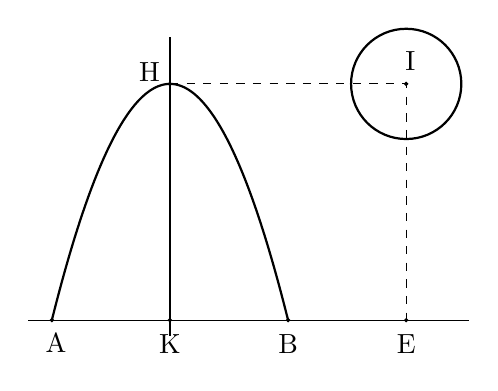
\begin{tikzpicture}[scale=0.1,>=stealth]
				% Axes
				\draw (-18,0)--(38,0);
				\draw (0,-2)--(0,36);
				
				% Parabola
				\draw[smooth,domain=-15:15,samples=200,thick]
				plot(\x,{-2*(\x)^2/15 + 30});
				
				% Circle
				\draw[thick] (30,30) circle (7);
				
				% Points
				\coordinate (A) at (-15,0);
				\coordinate (B) at (15,0);
				\coordinate (K) at (0,0);
				\coordinate (H) at (0,30);
				\coordinate (I) at (30,30);
				\coordinate (E) at (30,0);
				
				% Labels
				\foreach \x/\g in {A/-80,B/-90,K/-90,E/-90,H/150, I/80}
				\draw[fill=black] (\x) circle (0.2) +(\g:3) node{\x}
				;
				
				% Dashed lines
				\draw[dashed] (H)--(I)--(E);
			\end{tikzpicture}}
	\shortans{$20{,}6$}
	\loigiai{
		Chọn hệ trục tọa độ $Oxy$ sao cho gốc tọa độ $O\equiv K$, trục $Ox$ trùng với đường thẳng $AB$, trục $Oy$ trùng với đường thẳng $KH$.\\
		Khi đó,
		$K(0;0$), $H(0;30)$.\\
		Vì $AB=30$ và $K$ là trung điểm của $AB$ nên $A(-15;0)$, $B(15;0)$.\\
		Giả sử Parabol $(P)$ có phương trình $y=ax^2+30$.\\
		Vì $B(15;0)\in (P)$ nên $225a+30=0\Rightarrow a=-\dfrac{2}{15}$.\\		
		Do đó phương trình Parabol là $(P):\ y=-\dfrac{2}{15}x^2+30$, $x\in[-15;15]$.\\
		Theo giả thiết $IH=30$, $IE=30$ nên $I(30;30)$ và
		đường tròn $(C)$ có phương trình là:
		\[
		 (x-30)^2+(y-30)^2=9.
		\]		
		Gọi	$M\left(x;-\dfrac{2}{15}x^2+30\right)\in(P)$.
		Khi đó:
		$$
			MI^2
			=(x-30)^2+\left(-\frac{2}{15}x^2\right)^2
			=(x-30)^2+\frac{4x^4}{225}.
		$$		
		Xét hàm số $f(x)=\dfrac{4x^4}{225}+(x-30)^2$
		trên đoạn $[-15;15]$.	
		Ta có,	$f'(x)=\dfrac{16x^3}{225}+2x-60$.
		Giải phương trình:
		\[
		f'(x)=0
		\Leftrightarrow 16x^3+450x-13500=0\Rightarrow
		x\approx 8{,}4613.
		\]		
		Khi đó
		$MI_{\min}=\sqrt{f(8{,}4613)}\approx 23{,}559$.		
		Khoảng cách nhỏ nhất giữa hai bạn là:
		\[
		d_{\min}=MI_{\min}-R
		\approx 23{,}559-3
		=20{,}559\approx 20{,}6.
		\]
	}
\end{ex}
\begin{ex}%[2H2C2-6]
	Trong bản thiết kế của dự án lắp đặt đường dây điện cho vùng núi tỉnh $A$, các kĩ sư thiết kế các trụ điện cao $120\,\text{m}$. Để giữ thăng bằng cho trụ điện, người ta kéo dây cáp nối từ đỉnh trụ $S$ xuống mặt đất tại các điểm $A,B,C$ sao cho $S.ABC$ là hình chóp tam giác đều, khoảng cách từ chân trụ đến các điểm tiếp đất bằng $40\sqrt{3}\,\text{m}$. Tuy nhiên trong thực tế, do sườn núi dốc $10^\circ$ so với mặt biển nên vị trí tiếp đất của dây cáp tại $A,B',C'$ (với $BB'$, $CC'$ song song thân trụ điện, tham khảo hình vẽ). 
	\begin{center}
	 	\begin{tikzpicture}[line join=round,line cap=round,line width=.6pt,font=\footnotesize,scale=.5]
	 	\path 
	 	(0:0) coordinate (O)
	 	(90:8) coordinate (S)
	 	(0:6) coordinate (A)
	 	($(A)!1.5!(O)$)coordinate (H)
	 	($(H)+(30:5)$) coordinate (C)
	 	($(C)!2!(H)$)coordinate (B)
	 	($(B)-(0,1)$)coordinate (B')
	 	($(C)+(0,1)$)coordinate (C')
	 	($(A)!0.67!(B)$)coordinate (X)
	 	;
	 	
	 	\draw (S)--(B')--(B)--(S)--(A)--(B);
	 	\draw[dashed] (C)--(S)--(C')(A)--(O)--(S) (A)--(C)--(B) (B')--(C')--(C) (H)--(O)--(X);
	 	\draw[->] (S)--($(O)!1.3!(S)$)node[above]{$z$};
	 	\draw[->] (X)--($(O)!2.8!(X)$)node[below]{$x$};
	 	\draw[->] (A)--($(O)!1.2!(A)$)node[right]{$y$};
	 	% Labels
	 	\foreach \x/\g in {O/30,A/-80,B/180,C/-90,S/130,C'/0,B'/180,H/160}
	 	\draw[fill=black] (\x) circle (0.03) +(\g:0.5) node{\x}
	 	;
	 	\pic[draw,angle radius=1cm]{angle = C--H--C'};
	 	\draw($(H)+(0.8,1.2)$)node{$10^\circ$};
	 \end{tikzpicture}
	\end{center}
	Chọn hệ trục tọa độ $Oxyz$ với $O$ là chân trụ điện, mặt phẳng $(Oxy)$ song song với mặt biển, điểm $A$ thuộc tia $Oy$, trục $Oz$ hướng lên trên. Khi đó, tổng độ dài của ba dây cáp $SA$, $SB'$, $SC'$ bằng bao nhiêu? (Kết quả làm tròn đến hàng đơn vị mét.)
	\shortans{$416$}
	\loigiai{
		Đặt hệ trục tọa độ như đề bài. Khi đó:
		$O(0;0;0)$, $S(0;0;120)$.
		Vì $A,B,C\in (Oxy)$ và
		$
		OA=OB=OC=40\sqrt3,
		$
		nên	$A(0;40\sqrt3;0)$.\\		
		Gọi $B(x;y;0)$, $C(x';y';0)$.\\
		Do $O$ là tâm của $\triangle ABC$ đều và $A\in Oy$ nên $B,C$ đối xứng nhau qua trục $Oy$. Do đó,
		$x'=-x$, $y'=y$ và 
		$\dfrac{0+x+(-x)}3=0$,
		$
		\dfrac{40\sqrt3+y+y}{3}=0
		\Rightarrow 2y=-40\sqrt3
		\Rightarrow y=-20\sqrt3$.\\	
		Mặt khác:
		\[
		OB=40\sqrt3
		\Rightarrow x^2+(-20\sqrt3)^2=(40\sqrt3)^2.
		\Rightarrow
		x^2+1200=4800
		\Rightarrow x^2=3600
		\Rightarrow x=60.
		\]		
		Do đó
		$B(60;-20\sqrt3;0)$, 
		$C(-60;-20\sqrt3;0)$.\\
		Vì sườn núi dốc góc $10^\circ$ nên
		$
		BB'=CC'=60\tan10^\circ.
		$
		\\
		Suy ra:
		$B'(60;-20\sqrt3;-60\tan10^\circ)$.
		\\		
		Tương tự		
		$C'(-60;-20\sqrt3;60\tan10^\circ)$.
		\\
		Tính độ dài các dây cáp:\\
	$\begin{aligned}
		SA
		&=
		\sqrt{(40\sqrt3)^2+120^2}
		=
		40\sqrt{12}
		=
		80\sqrt3.
	\\
			SB'
			&=\sqrt{	60^2+(-20\sqrt3)^2+\left(120+60\tan10^\circ\right)^2}=\sqrt{	4800+\left(120+60\tan10^\circ\right)^2},
			\\
			SC'
			&=\sqrt{(-60)^2+(-20\sqrt3)^2+\left(120-60\tan10^\circ\right)^2}=\sqrt{4800+\left(120-60\tan10^\circ\right)^2}.
		\end{aligned}$\\	
		Vậy\\
		$\begin{aligned}
			SA+SB'+SC'
			&=80\sqrt{3}+\sqrt{4800+\left(120+60\tan10^\circ\right)^2}+\sqrt{4800+\left(120-60\tan10^\circ\right)^2}
			\\
			& \approx 416.
		\end{aligned}$
	}
\end{ex}
\Closesolutionfile{ans}
\indapan{6}{ans/ans-OTTNTHPT-DE27-KQ}